% !TEX root =  ../main_manuscript.tex 
\section{Results}
\subsection{Joint Model Results}
\textbf{Overall cumulative-risk:} In PRIAS, the probability of experiencing reclassification within the first five and ten years was 33\% and 42\%, respectively (cumulative-risk plot in Appendix A). That is, many patients do not require any biopsy in the first ten years.

\textbf{Effect of age at inclusion in AS:} For every ten year increase in patient age, the adjusted hazard ratio of reclassification is 1.45~(95\%CI:~1.30--1.63). 

\textbf{Effect of PSA:} When PSA value (log scale) increases from 2.36 to 3.07 (25-th and 75-th percentile of fitted PSA), the adjusted hazard ratio of reclassification is 0.99~(95\%CI:~0.89--1.11). When estimated instantaneous PSA (log scale) velocity increases from -0.09 to 0.31 (25-th and 75-th percentile of estimated velocity), the adjusted hazard ratio of reclassification is 2.47~(95\%CI:~1.93--2.99). Hence, instantaneous PSA (log scale) velocity is a stronger predictor for reclassification than PSA value (log scale). Detailed parameter estimates are in Appendix~A.4.

\subsection{Validation Results}
\textbf{Discrimination (AUC):} Since AS studies are longitudinal in nature, the area under the receiver operating characteristic curve (AUC) changes over time. This time-varying AUC is shown in Panel~A, Figure~\ref{fig:auc_calib}. The AUC is only calculated until year five (95-percentile of observed reclassification times in PRIAS) of follow-up. 

\textbf{Calibration:} The calibration plots in Panel~B, Figure~\ref{fig:auc_calib} indicate that the model predictions are well calibrated for all five external cohorts. 

Detailed results for model validation are available in Appendix B.
%For predictions within PRIAS (internal validation), the time-dependent AUC was between 0.62 and 0.69, and RMSPE between 0.23 and 0.37 over the whole follow-up period. For validation in external cohorts, the AUC was similar to the AUC of PRIAS for all cohorts during the first three years of follow-up. 

\begin{figure}
\centerline{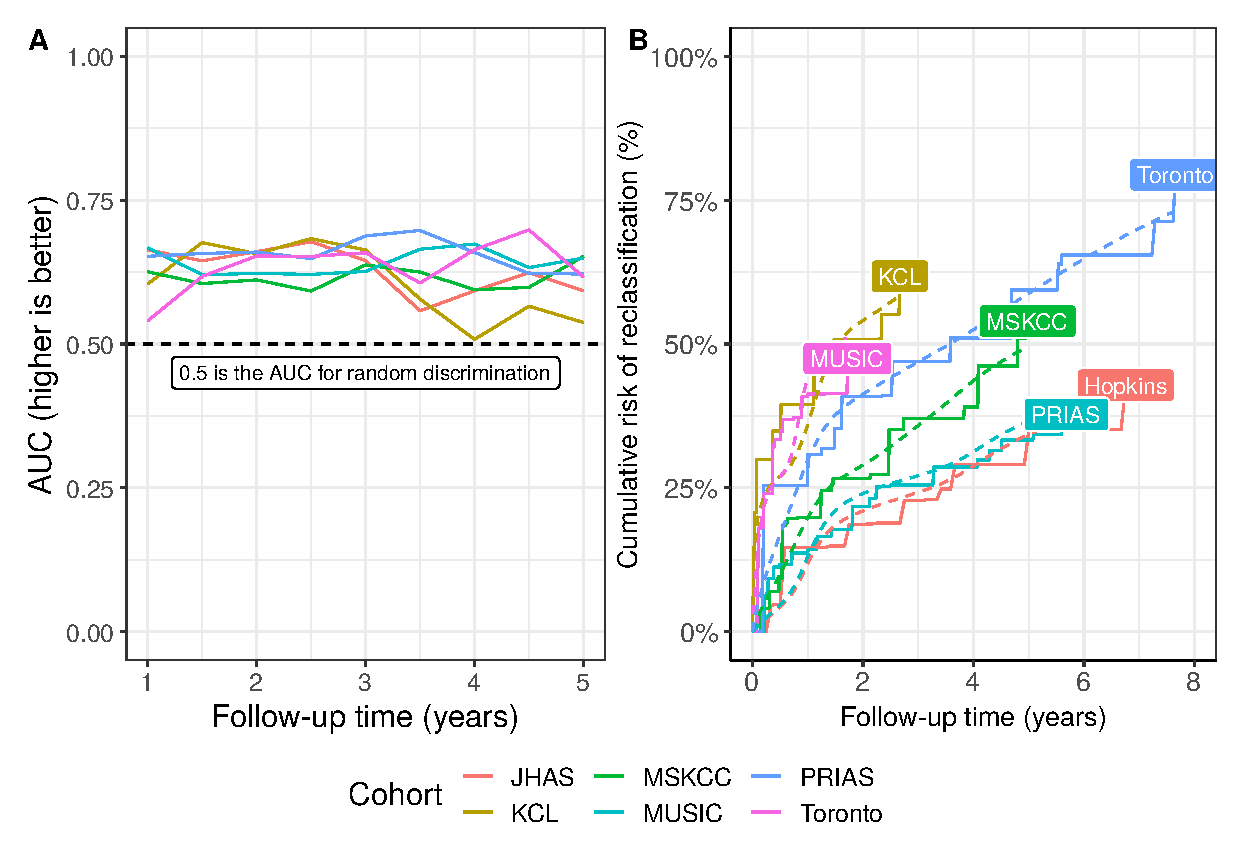
\includegraphics[width=\columnwidth]{images/auc_calib.eps}}
\caption{\textbf{Validation of predictions of Gleason $\geq$ 7 (GS7)}. In \textbf{Panel~A} we can see that the time dependent area under the receiver operating characteristic curve or AUC (measure of discrimination) is above 0.5 in PRIAS (internal validation), and in Toronto, JHAS, MSKCC, KCL, and MUSIC AS cohorts (external validation). In \textbf{Panel~B} we can see that the time dependent root mean squared prediction error or RMSPE (measure of calibration) is similar for PRIAS, and JHAS and Toronto cohorts. The bootstrapped 95\% confidence interval for these estimates are presented in Table 6 to Table 11 of Appendix B. Full names of Cohorts are \textit{PRIAS}: Prostate Cancer International Active Surveillance, \textit{Toronto}: University of Toronto Active Surveillance, \textit{JHAS}: Johns Hopkins Active Surveillance, \textit{MSKCC}: Memorial Sloan Kettering Cancer Center Active Surveillance, \textit{KCL}: King's College London Active Surveillance, \textit{MUSIC}: Michigan Urological Surgery Improvement Collaborative Active Surveillance.}
\label{fig:auc_calib}
\end{figure}

\subsection{Personalized Schedule Results}
Various personalized and fixed biopsy schedules for demo patients are shown in Figure \ref{fig:demo_pat1} 

In addition, we scheduled biopsies only for the first ten years follow-up because of limited follow-up period of the training dataset PRIAS. A compulsory biopsy was done scheduled year ten of follow-up in all schedules for meaningful comparison of their expected delays in detection of GS7. and Appendix C's Figure 6, 7, 8 and 9. The biopsies denoted by `B' show that personalized schedules schedule fewer biopsies than fixed schedules. At the same time the expected time delay in detection of GS7 is less than an year for personalized schedules. We have implemented this approach in a web-application (\url{https://emcbiostatistics.shinyapps.io/prias_biopsy_recommender/}, and Appendix D) for practical use.